\documentclass{article}
\usepackage{lingmacros}
\usepackage[danish]{babel}
\usepackage{enumitem}
\usepackage{lmodern}
\usepackage[utf8]{inputenc}
\usepackage[T1]{fontenc}
\usepackage{color}
\usepackage{amssymb}
\usepackage{listings}
\usepackage{listingsutf8}
\usepackage{color} %red, green, blue, yellow, cyan, magenta, black, white
\definecolor{mygreen}{RGB}{28,172,0} % color values Red, Green, Blue
\definecolor{mylilas}{RGB}{170,55,241}
\lstset{literate=
  {æ}{{\ae}}{1} 
  {å}{{\aa}}{1} 
  {ø}{{\o}}{1} }
\usepackage{graphicx}
\usepackage[export]{adjustbox}
\usepackage{fullpage}
\lstset{basicstyle=\ttfamily,breaklines=true}
% \lstset{framextopmargin=50pt,frame=bottomline}
\lstset{
% numbers=left, 
% numberstyle=\small, 
% numbersep=8pt, 
frame = single, 
language=Pascal, 
framexleftmargin=15pt}
\usepackage[T1]{fontenc}
\usepackage[hidelinks]{hyperref}
% \usepackage{maplestd2e}
\usepackage{tree-dvips}
% \usepackage{biblatex}
% \usepackage[style=verbose,backend=bibtex]{biblatex}
% \bibliography{oeve1dsb.bib}
% \usepackage{sagetex}
\usepackage{amsmath}
% \usepackage{newpxtext,newpxmath}
\usepackage{courier}
\linespread{1.5}
\makeatletter
\renewcommand*\env@matrix[1][*\c@MaxMatrixCols c]{%
  \hskip -\arraycolsep
  \let\@ifnextchar\new@ifnextchar
  \array{#1}}
\makeatother
\title{E4DSA\\ Case projekt 2 – audio IIR notch filter}
\author{Team 8}
\def\emptyline{\vspace{12pt}}

\begin{document}
%\newcommand{\includecode}[2][c]{\lstinputlisting[caption=#2, escapechar=, style=custom#1]{#2}<!---->}
\lstset{language=Matlab,%
    %basicstyle=\color{red},
    breaklines=true,%
    morekeywords={matlab2tikz},
    keywordstyle=\color{blue},%
    morekeywords=[2]{1}, keywordstyle=[2]{\color{black}},
    identifierstyle=\color{black},%
    stringstyle=\color{mylilas},
    commentstyle=\color{mygreen},%
    showstringspaces=false,%without this there will be a symbol in the places where there is a space
    % numbers=left,%
    % numberstyle={\tiny \color{black}},% size of the numbers
    % numbersep=9pt, % this defines how far the numbers are from the text
    emph=[1]{for,end,break},emphstyle=[1]\color{red}, %some words to emphasise
    %emph=[2]{word1,word2}, emphstyle=[2]{style},    
  }
\maketitle
\tableofcontents
\newpage

\section{Opgave}
\label{sec:opgave}

\subsection{puls}
\label{sec:puls}

\begin{figure}[h!]
  \centering
  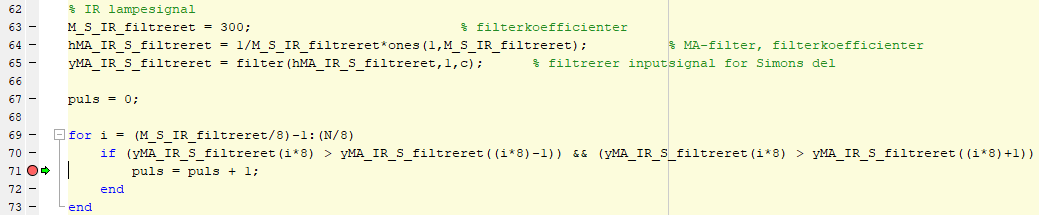
\includegraphics[width=1.0\textwidth]{billeder/breakpoint.png}
  \caption{breakpoints opfanget for hver puls inkrementering}
  \label{fig:breakpoint}
\end{figure}

der ses på billede \ref{fig:breakpoint} hvordan der er sat et breakpoint hver gang puls variablen bliver inkrementeret, dette sker når henholdsvist 8 tidligere samples er lavere, samme tid med 8 næste samples er højere.
Tanken her var at det i praksis betyder der er nået toppen af kurven der er sidst påsatte MA filter.

\begin{figure}[h!]
  \centering
  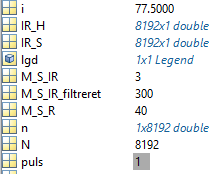
\includegraphics[width=0.4\textwidth]{billeder/break1.png}
  \caption{første breakpoint}
  \label{fig:break1}
\end{figure}

\begin{figure}[h!]
  \centering
  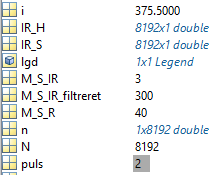
\includegraphics[width=0.4\textwidth]{billeder/break2.png}
  \caption{andet breakpoint}
  \label{fig:break2}
\end{figure}

\begin{figure}[h!]
  \centering
  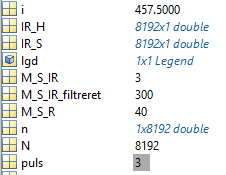
\includegraphics[width=0.4\textwidth]{billeder/break3.png}
  \caption{tredje breakpoint}
  \label{fig:break3}
\end{figure}

\begin{figure}[h!]
  \centering
  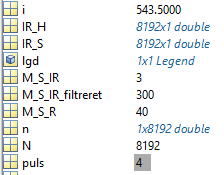
\includegraphics[width=0.4\textwidth]{billeder/break4.png}
  \caption{fjerde breakpoint}
  \label{fig:break4}
\end{figure}

der ses på billede \ref{fig:break1} \ref{fig:break2} \ref{fig:break3} samt \ref{fig:break4} de 4 første breakpoints fanget, der er lagt dokumentation for alle 11 breakpoints op på git.

\begin{figure}[h!]
  \centering
  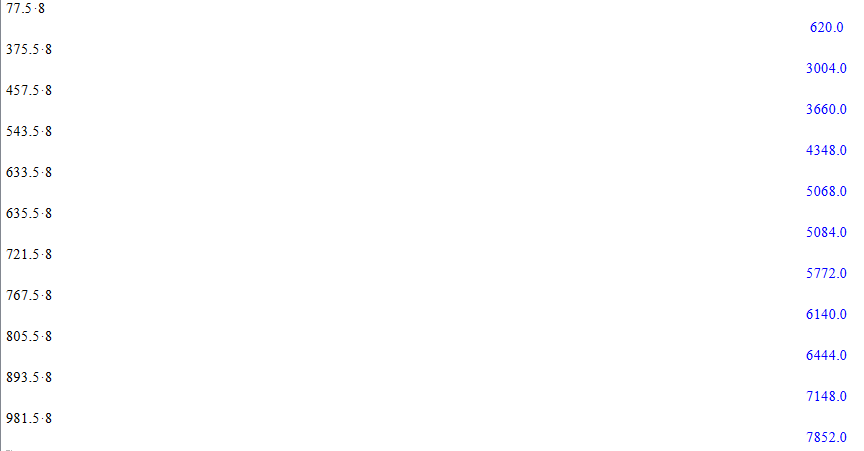
\includegraphics[width=0.8\textwidth]{billeder/udregning.png}
  \caption{breakpoints omregnet}
  \label{fig:udregning}
\end{figure}

\begin{figure}[h!]
  \centering
  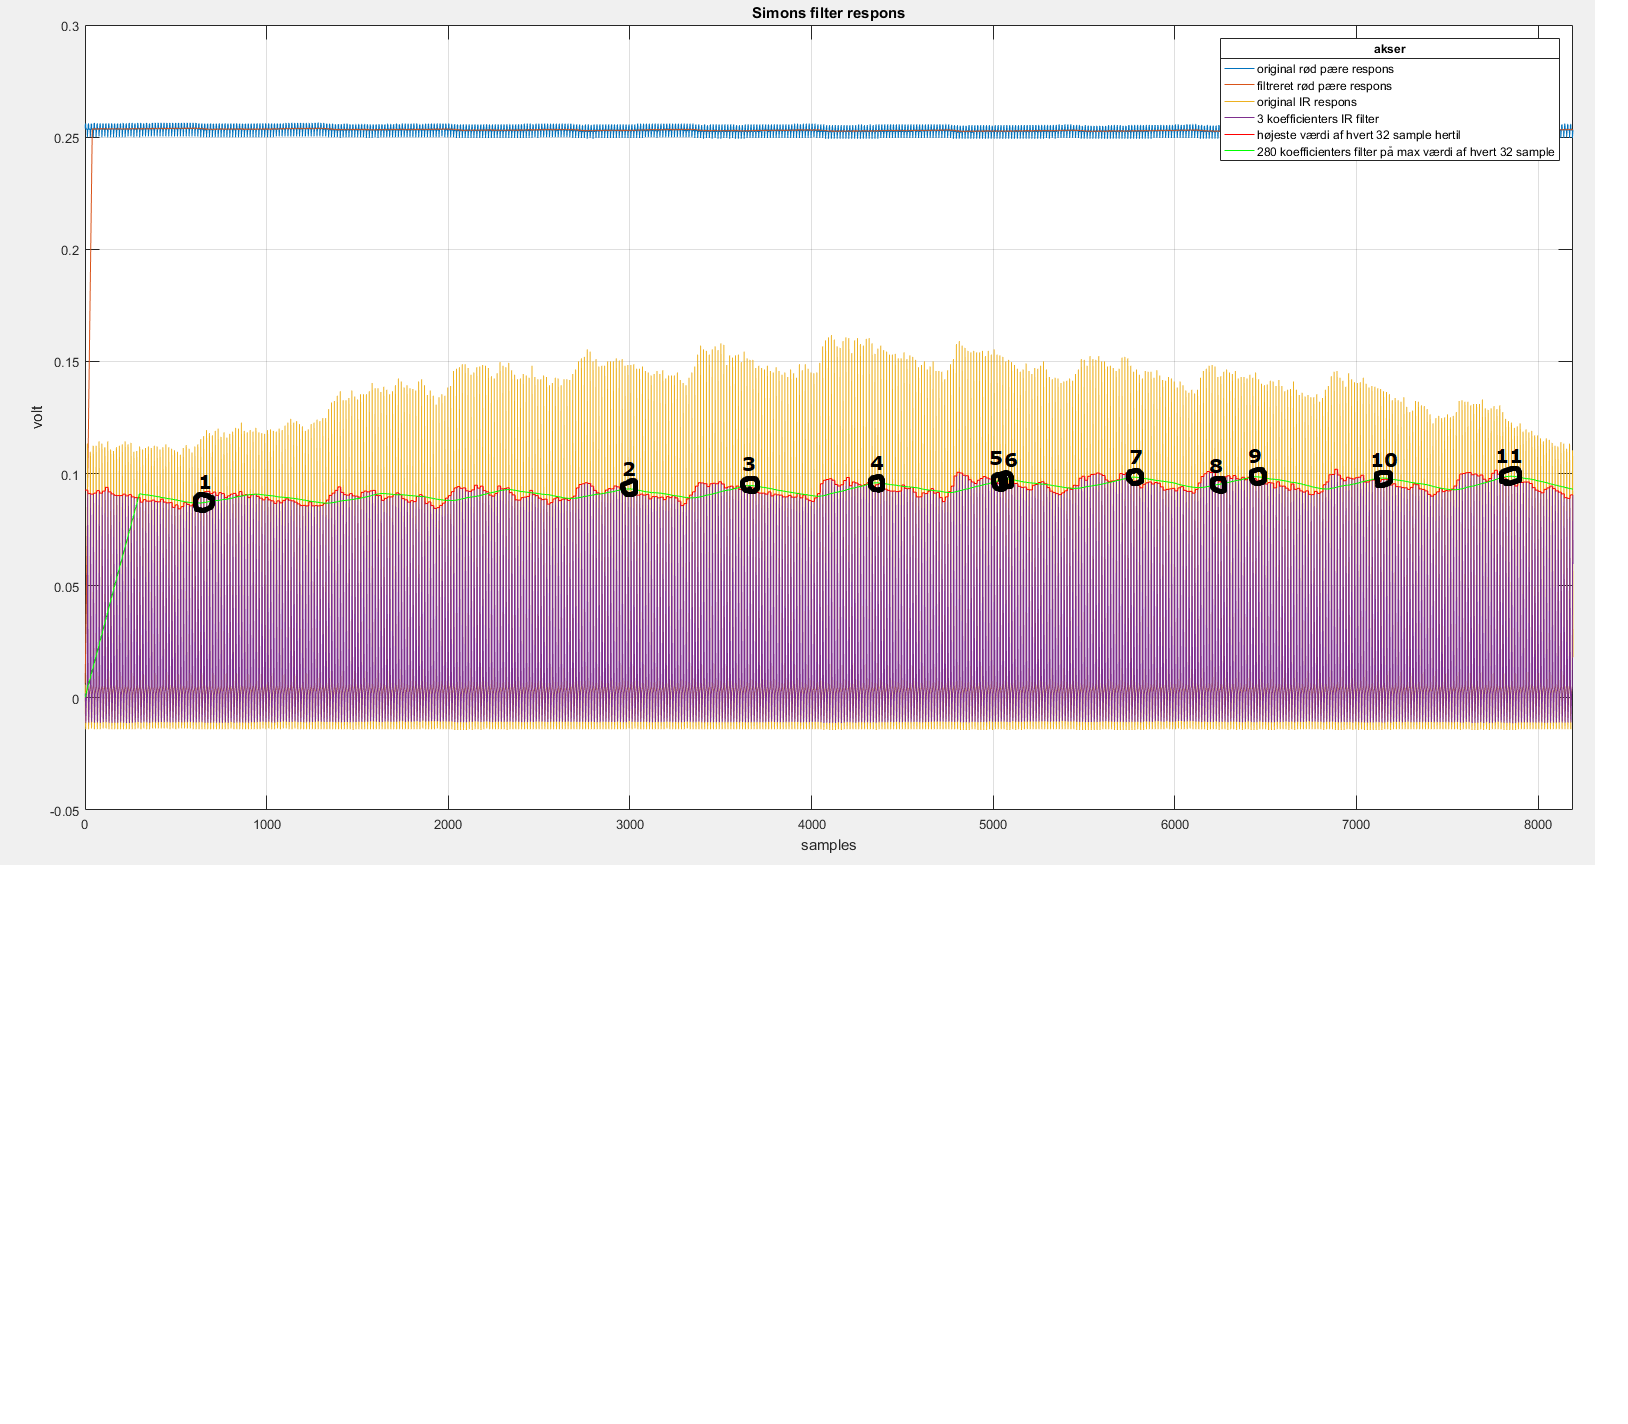
\includegraphics[width=1.0\textwidth]{billeder/punkter.png}
  \caption{punkter indtegnet}
  \label{fig:punkter}
\end{figure}

billede \ref{fig:udregning} viser alle 11 breakpoints ganget med 8 for at kunne se hvilket nummer sample disse var i praksis, disse er herefter tegnet ind på billede \ref{fig:punkter} 


\end{document}
